\section{Aufgabenstellung}
Ziel dieses Versuchs ist die Bestimmung der mittleren Lebensdauer des $^{3}P_{1}$-Zustands von Quecksilber mittels des Hanle-Effekts. Mehrfache Resonanzfluoreszenz ('Coherence Narrowing') lässt die Lebensdauer länger erscheinen, weshalb bei unterschiedlichen Drücken gemessen werden muss, um durch Extrapolation auf den tatsächlichen Wert schließen zu können.
\section{Theoretische Grundlagen}
\subsection{Hanle-Effekt: semiklassische Beschreibung}
Ein Atom, welches ein Photon absorbiert, kann ab dem Zeitpunkt der Absorption als oszillierender Dipol betrachtet werden. Dessen Achse ist parallel zur Polarisationsrichtung des absorbierten Photons.
\begin{center}
\begin{figure}[htbp]
\hspace{4.0cm}
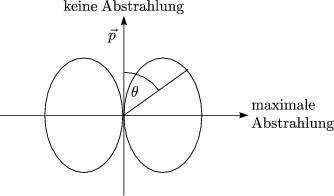
\includegraphics{Bilder/dipol}
\caption{Dipol mit eingezeichnetem Beobachtungswinkel $\theta$ sowie der zur Polarisationsrichtung des absorbierten Photons parallelen Achse $\vec{p}$. Quelle:[uka].}
\end{figure}
\end{center}
Die Abstrahlung ist proportional zu $\sin^{2}(\theta)$. Außerdem wird über einen Faktor $e^{-\frac{t}{\tau}}$ das Zurückfallen des angeregten Elektrons in den Grundzustand beschrieben ($\tau$ steht dabei für die Lebensdauer des angeregten Zustands). Die Gesamtintensität ergibt sich dann als Integral über alle Zeiten: \[I=C\cdot\int_{0}^{\infty}\sin^{2}(\theta)\cdot e^{-\frac{t}{\tau}}dt\] 
Wird ein zur Oszillationsbewegung senkrechtes Magnetfeld angelegt, so führt dies zu einem Drehmoment und damit zu einer Präzessionsbewegung senkrecht zur magnetischen Flussdichte $\vec{B}$. Wird das Dipolmoment und das magnetische Moment $\vec{\mu}$ als starr verbunden betrachtet, so präzedieren beide und man erhält folgende Bewegungsgleichung: \[\frac{d\vec{\mu}}{dt}=\frac{\omega_{L}}{B}\cdot(\vec{\mu}\times\vec{B})\]
mit $B=\left|\vec{B}\right|$ und der 'Larmorfrequenz' $\omega_{L}=g_{J}\cdot\frac{\mu_{B}}{\hbar}B$. Die in dieser Formel vorkommenden Größen sind
\begin{itemize}
\item das reduzierte Plancksche Wirkungsquantum $\hbar=\frac{h}{2\pi}$;
\item der 'Landé-Faktor' $g_{J}=1+\frac{J\cdot(J+1)-L\cdot(L+1)+S\cdot(S+1)}{2J\cdot(J+1)}$, wobei S die Summe der Elektronenspins, L die Summe der Bahndrehimpuls-Quantenzahlen und $J=L+S~bzw.~L-S$ für mehr als halbvolle bzw. weniger als halbvolle Schalen ist;
\item das Bohrsche Kernmagneton $\mu_{B}=\frac{e\cdot\hbar}{2m_{e}}$ mit der Elektronenladung e und der Elektronenmasse $m_{e}$.
\end{itemize}
Die Präzessionsbewegung eines Elektrons mit Dipolmoment $\vec{P}$, Drehimpuls $\vec{L}$, magnetischem Moment $\vec{\mu_{L}}$ und einem auf es wirkenden Magnetfeld der Flussdichte $\vec{B}$ kann man sich durch folgende Skizze verdeutlichen:
\begin{center}
\begin{figure}[h]
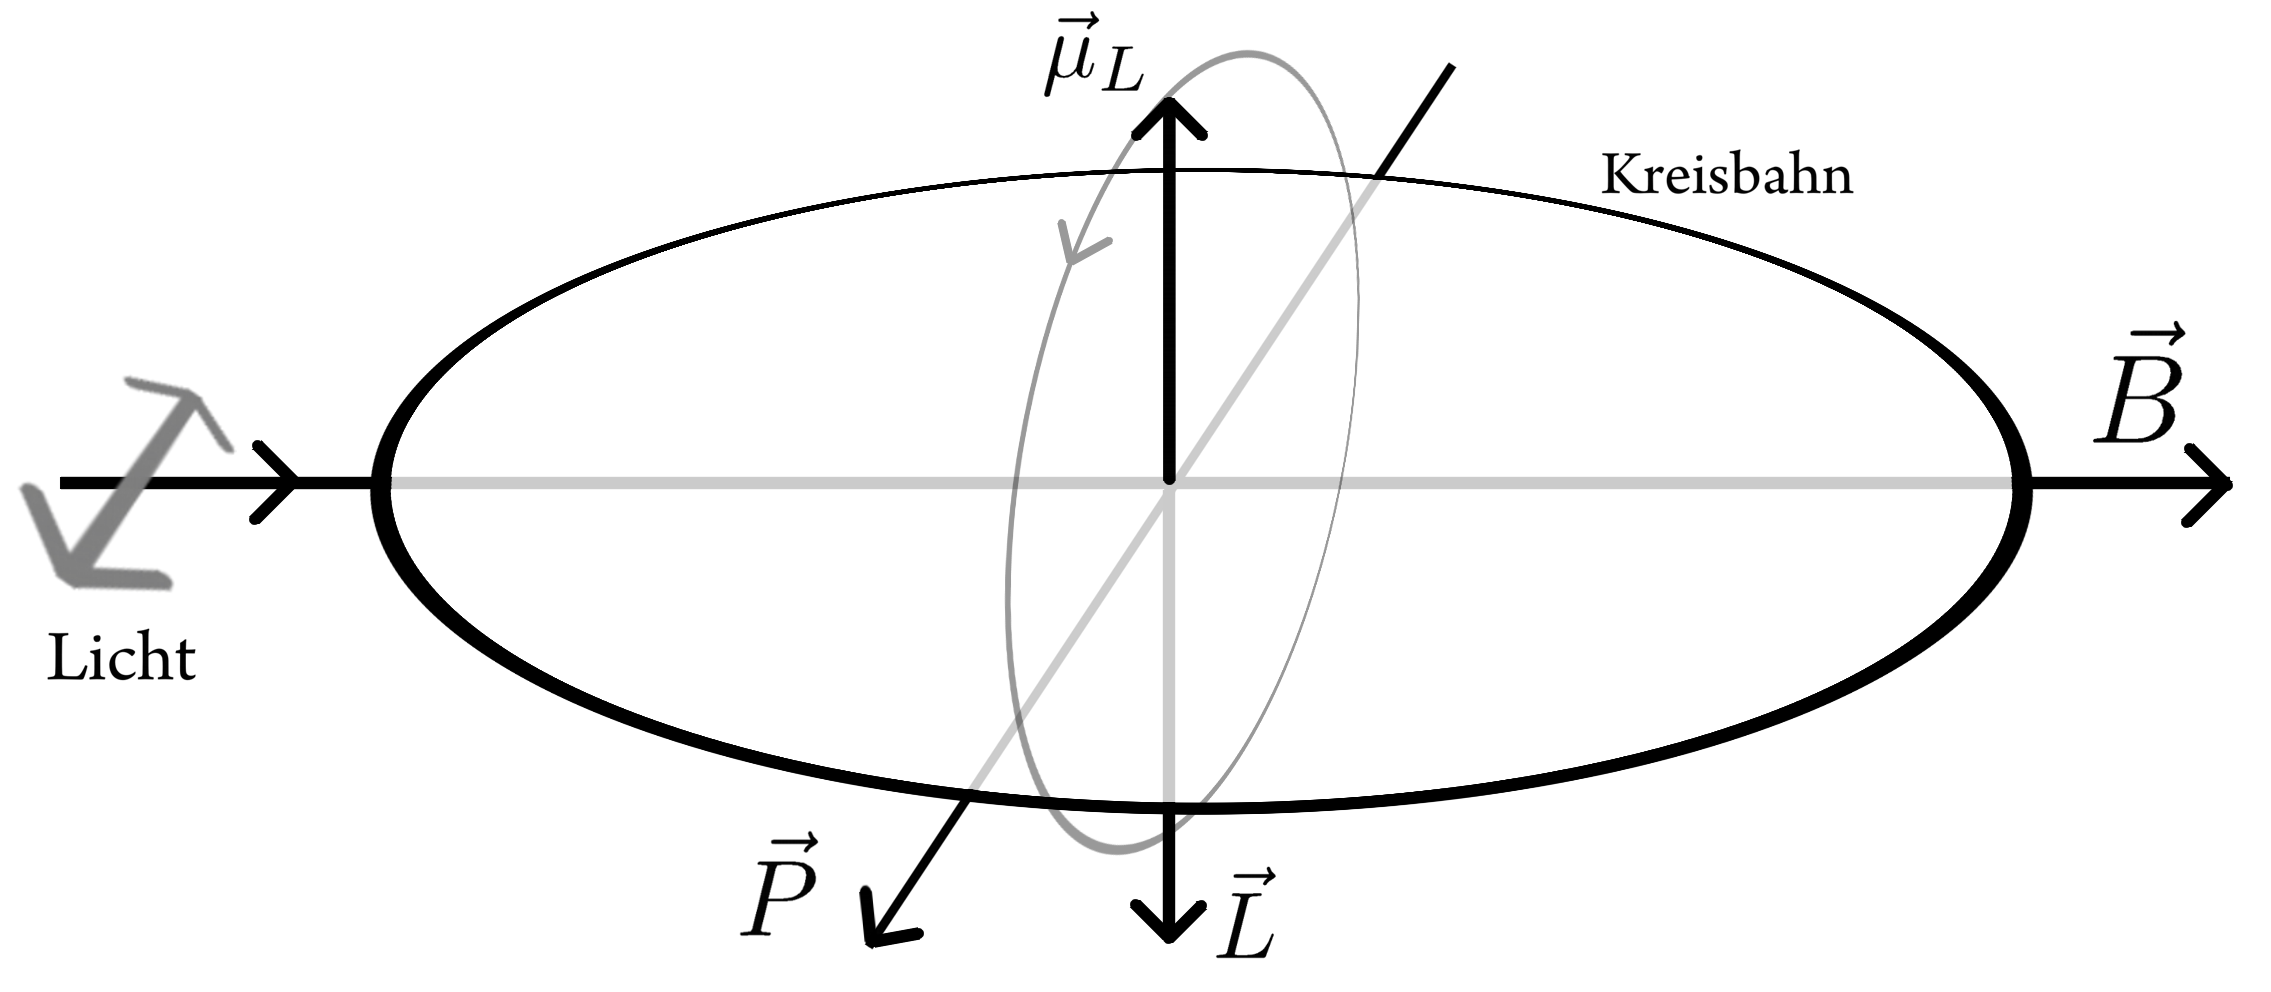
\includegraphics[scale=0.3]{Bilder/praezession}
\caption{Präzessionsbewegung eines Elektrons. Quelle:[ver].}
\end{figure}
\end{center}
Zur weiteren Betrachtung wird das kartesische Koordinatensystem so gelegt, dass die Probe im Ursprung, die einfallende Strahlung in der x-Achse und der Detektor in der y-Achse liegt. \\
Beträgt der Winkel zur z-Achse $90^{\circ}$, so spricht man von einer $90^{\circ}$-Konfiguration, welche eine zur Beobachtungsrichtung parallele Polarisation (und somit Dipolachse) darstellt. Für diese Einstellung gilt $\theta(t)=\omega_{L}\cdot t$, wodurch man für die Intensität eine invertierte Lorentzkurve erhält: \[I=C\cdot\int_{0}^{\infty}\sin(\omega_{L}t)^{2}\cdot e^{-\frac{t}{\tau}}dt=C\cdot\frac{\tau}{2}\left(\frac{(2\omega_{L}\tau)^{2}}{1+(2\omega_{L}\tau)^{2}}\right).\]
Ist die Polarisation senkrecht zur Beobachtungsrichtung, so spricht man von der $0^{\circ}$-Konfiguration, für welche $\theta(t)=\omega_{L}t+\frac{\pi}{2}$ gilt. Für diese erhält man eine normale Lorentzkurve für den Intensitätsverlauf: \[I=C\cdot\int_{0}^{\infty}\cos(\omega_{L}t)^{2}e^{-\frac{t}{\tau}}dt=C\cdot\frac{\tau}{2}\left(2-\frac{(2\omega_{L}\tau)^{2}}{1+(2\omega_{L}\tau)^{2}}\right).\]
Berücksichtigt man, dass $\omega_{L}\propto B$ gilt, so ist es klar dass die Intensität in Abhängigkeit vom angelegten B-Feld bestimmt werden kann. \\
Die Lebensdauer $\tau$ wird über die volle Halbwertsbreite (FWHM) der Lorentzkurve, $B_{FW}$, ermittelt, da bei der Hälfte des Maximums der Intensität folgendes gilt: \[\tau=\frac{\hbar}{g_{J}\mu_{B} B_{FW}}.\]
\begin{center}
\begin{figure}[h]
\hspace{1.5cm}
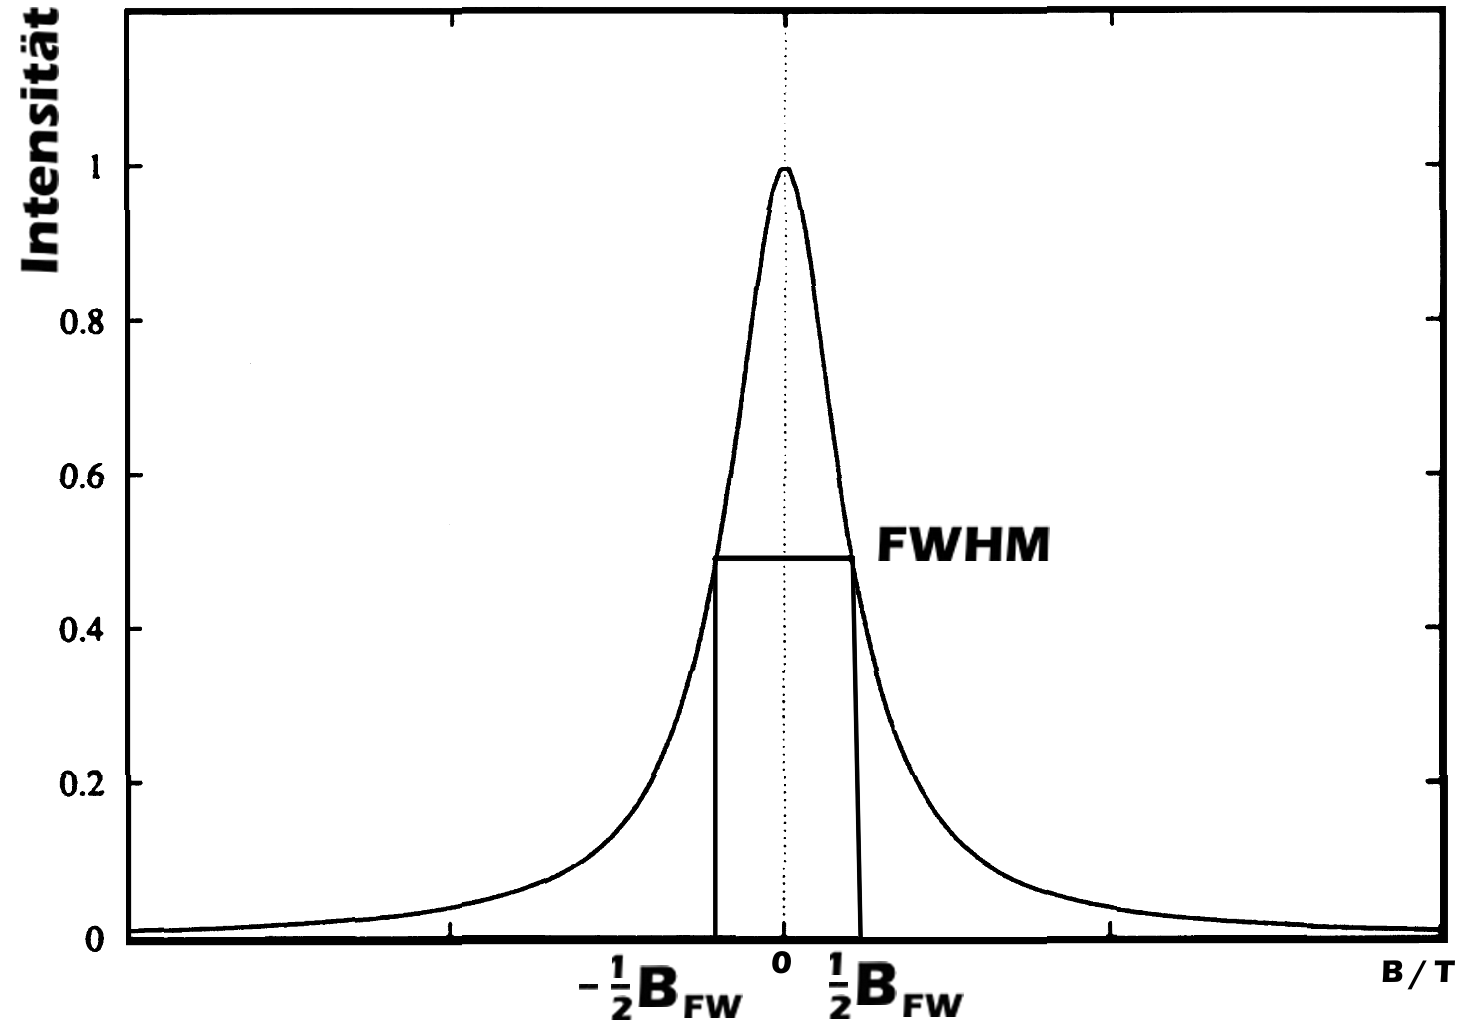
\includegraphics[scale=0.3]{Bilder/fwhm}
\caption{Lorentzkurve bei $0^{\circ}$-Konfiguration. Quelle:[ver].}
\end{figure}
\end{center}
~\\
\subsection{Hanle-Effekt: quantenmechanische Beschreibung}
Betrachtet man den Hanle-Effekt quantenmechanisch, so stellt er einen Spezialfall des sogenannten 'level-crossing' dar. Unter diesem Effekt versteht man, dass bei Anlegen eines äußeren Magnetfeldes die schon vorhandene Zeeman-Aufspaltung weiter aufgespalten wird, sodass sich dadurch einzelne Niveaus überkreuzen können (dieses Phänomen wird als Entartung bezeichnet). Der Hanle-Effekt ist ein Spezialfall des sogenannten 'level-crossing' bei einem Magnetfeld mit dem Fluss $B=0T$. Die entarteten Zustände sind energetisch gleich und können daher kohärent angeregt werden. Bei der Abregung dieser Zustände kommt es zur Interferenz. Aus diesem Grund ist die beobachtete Intensität proportional zum Quadrat der Summe der Amplituden $(A_{1}+A_{2})^{2}$. Durch die Kohärenz ist die spektrale Auflösung nicht durch den Doppeleffekt beschränkt, sondern nur durch die natürliche Linienbreite, welche direkt mit der Lebensdauer des Zustands verknüpft ist.
\subsubsection{Breit-Formel}
Mithilfe der Breit-Formel, welche die Emissionsrate von Photonen einer linearen Polarisationsrichtung $\vec{g}$ beschreibt, wenn in Richtung $\vec{f}$ polarisiertes Licht eingestrahlt wird, werden somit Rückschlüsse auf den Intensitätsverlauf erlaubt. \\
Im Allgemeinen geht man von verschiedenen stabilen Grundzuständen $\ket{m}$ und angeregten Zuständen $\ket{\mu}$ aus. Das System ist für t<0s im Grundzustand und für $t=0s$ trifft ein Photon auf ein Atom der Probe, wobei der Hamiltonoperator der Wechselwirkung $H=-\vec{D}\cdot\vec{E}$ ($\vec{D}$: Dipoloperator, $\vec{E}$: Feldoperator) entspricht. Dabei ist der Dipoloperator proportional zum Ortsoperator $\vec{r}$ und der Feldoperator zu $\vec{f}$. Für die Wahrscheinlichlichkeitsamplitude eines Übergangs erhält man die Matrixelemente $f_{ba}=\bra{b}\vec{r}\cdot\vec{f}\ket{a}$. Die Probe befindet sich somit für $t>0s$ im Zustand \[\ket{\psi}=\ket{m}+\sum_{\mu}f_{\mu m}\ket{\mu}e^{(-i\omega_{\mu}+\Gamma_{\mu}/2)t}\]
Die Energie des Ausgangs-Grundzustandes ist der Nullpunkt und $\omega_{\mu}$ ist die Energie des angeregten Zustandes. Dissipative Prozesse sorgen für die Entstehung des Dämpfungsterms $\Gamma_{\mu}=\frac{1}{\tau_{\mu}}$, welcher die Lebensdauer $\tau_{\mu}$ des angeregten Zustandes $\ket{\mu}$ enthält.\\
Zum Zeitpunkt t erhält man als Übergangswahrscheinlichkeit, mit der Photonen der Polarisation $\vec{g}$ ausgesendet werden: \[R(\vec{f},\vec{g},t)=\sum_{mm'}\left|\bra{m'}\vec{r}\cdot\vec{g}\ket{\psi}\right|^{2}=\sum_{mm'}\sum_{\mu\mu'}f_{m\mu}f_{\mu'm}g_{\mu m'}g_{m'\mu'}e^{(i(\omega_{\mu}-\omega_{\mu'})-\Gamma_{\mu\mu'})t}\]
Hierbei gilt $g_{mm'}=g_{m'm}=0$ und $\Gamma_{\mu\mu'}=\frac{1}{2}(\Gamma_{\mu}+\Gamma_{\mu'})$ und zusätzlich wird über alle Anfangszustände m summiert. Für eine Bestrahlung mit N Photonen pro Sekunde ergibt sich somit als Gesamtrate: \[R(\vec{f},\vec{g})=N\int_{0}^{\infty}R(\vec{f},\vec{g},t)dt=N\sum_{mm'}\sum_{\mu\mu'}\frac{f_{m\mu}f_{\mu'm}g_{\mu m'}g_{m'\mu'}}{\Gamma_{\mu\mu'}-i(\omega_{\mu}-\omega_{\mu'})}.\]
\subsubsection{Anwendung in diesem Experiment}
Wir untersuchen den Übergang vom $^{3}P_{1}$- zum $^{1}S_{0}$-Zustand bei Quecksilber. Das bedeutet, dass es nur einen Grundzustand ($^{1}S_{0}$) gibt, während der $^{3}P_{1}$-Zustand durch das angelegte Magnetfeld in drei Terme mit den Quantenzahlen $m_{J}=-1,0,1$ aufgespaltet wird. Da nur Zustände zirkularer Polarisation in unserem Versuch eine Rolle spielen, kann $m_{J}=0$ vernachlässigt werden. \\
Zur Anwendung der Breitschen Formeln bezeichnen wir den Grundzustand mit a und die beiden angeregten Zustände mit b bzw. c. Somit erhalten wir folgende Gesamtrate: \[R=\frac{\left|f_{ab}\right|^{2}\left|g_{ba}\right|^{2}}{\Gamma_{b}}+\frac{f_{ab}f_{ac}g_{ca}g_{ab}}{\Gamma_{bc}-i(\omega_{b}-\omega_{c})}+\frac{f_{ab}f_{ca}g_{ca}g_{ba}}{\Gamma_{bc}-i(\omega_{c}-\omega_{b})}+\frac{\left|f_{ac}\right|^{2}\left|g_{ca}\right|^{2}}{\Gamma_{c}}\]
Über die Energie $\hbar\omega_{\mu}=m\cdot g_{J}\mu_{B}B$ eines Zeeman-Niveaus $\mu$ mit Quantenzahl m erhält man den Frequenzabstand von b ($m=-1$) und c ($m=1$) zu \[\Delta\omega=\omega_{c}-\omega_{b}=\frac{2g_{J}\mu_{B}B}{\hbar}=2\omega_{L}\]
Für schwache Magnetfelder hat R also die Form einer kohärenten Superposition: $R_{koh}\approx\left|f_{ab}g_{ba}+f_{ac}g_{ca}\right|^{2}$.\\
Gilt $\Delta\omega>>\Gamma_{bc}$, so handelt es sich hauptsächlich um eine nicht-kohärente Überlagerung (keine Interferenzterme): $R_{sep}\approx\left|f_{ab}\right|^{2}\left|g_{ba}\right|^{2}+\left|f_{ac}\right|^{2}\left|g_{ca}\right|^{2}$. \\
Benutzt man nun $f_{ba}f_{ac}g_{ca}g_{ab}=A$ und $\Gamma_{bc}=\Gamma$, so ergibt sich \[R=R_{sep}+\frac{A}{\Gamma+i\Delta\omega}+\frac{A^{\ast}}{\Gamma-i\Delta\omega}=R_{sep}+2Re(A)\cdot\frac{\Gamma}{\Gamma^{2}+\Delta\omega^{2}}\]
Mit dem bereits diskutierten Zusammenhang $\Gamma=\frac{1}{\tau}$ und $\Delta\omega=2\omega_{L}$ erhält man eine Lorentzkurve bekannter Form (bis auf Konstanten): \[R=C\frac{1}{1+(2\omega_{L}\tau)^{2}}\] 
\clearpage
\subsubsection{Beispiele für Hanle-Signale}
Für die unterschiedlichen Polarisatoreinstellungen von $0^{\circ}, 90^{\circ}$ und $45^{\circ}$ sollten Signale der folgenden Form entstehen (Quelle: [ver]):
\begin{center}
\begin{figure}[h]
\hspace{3.0 cm}
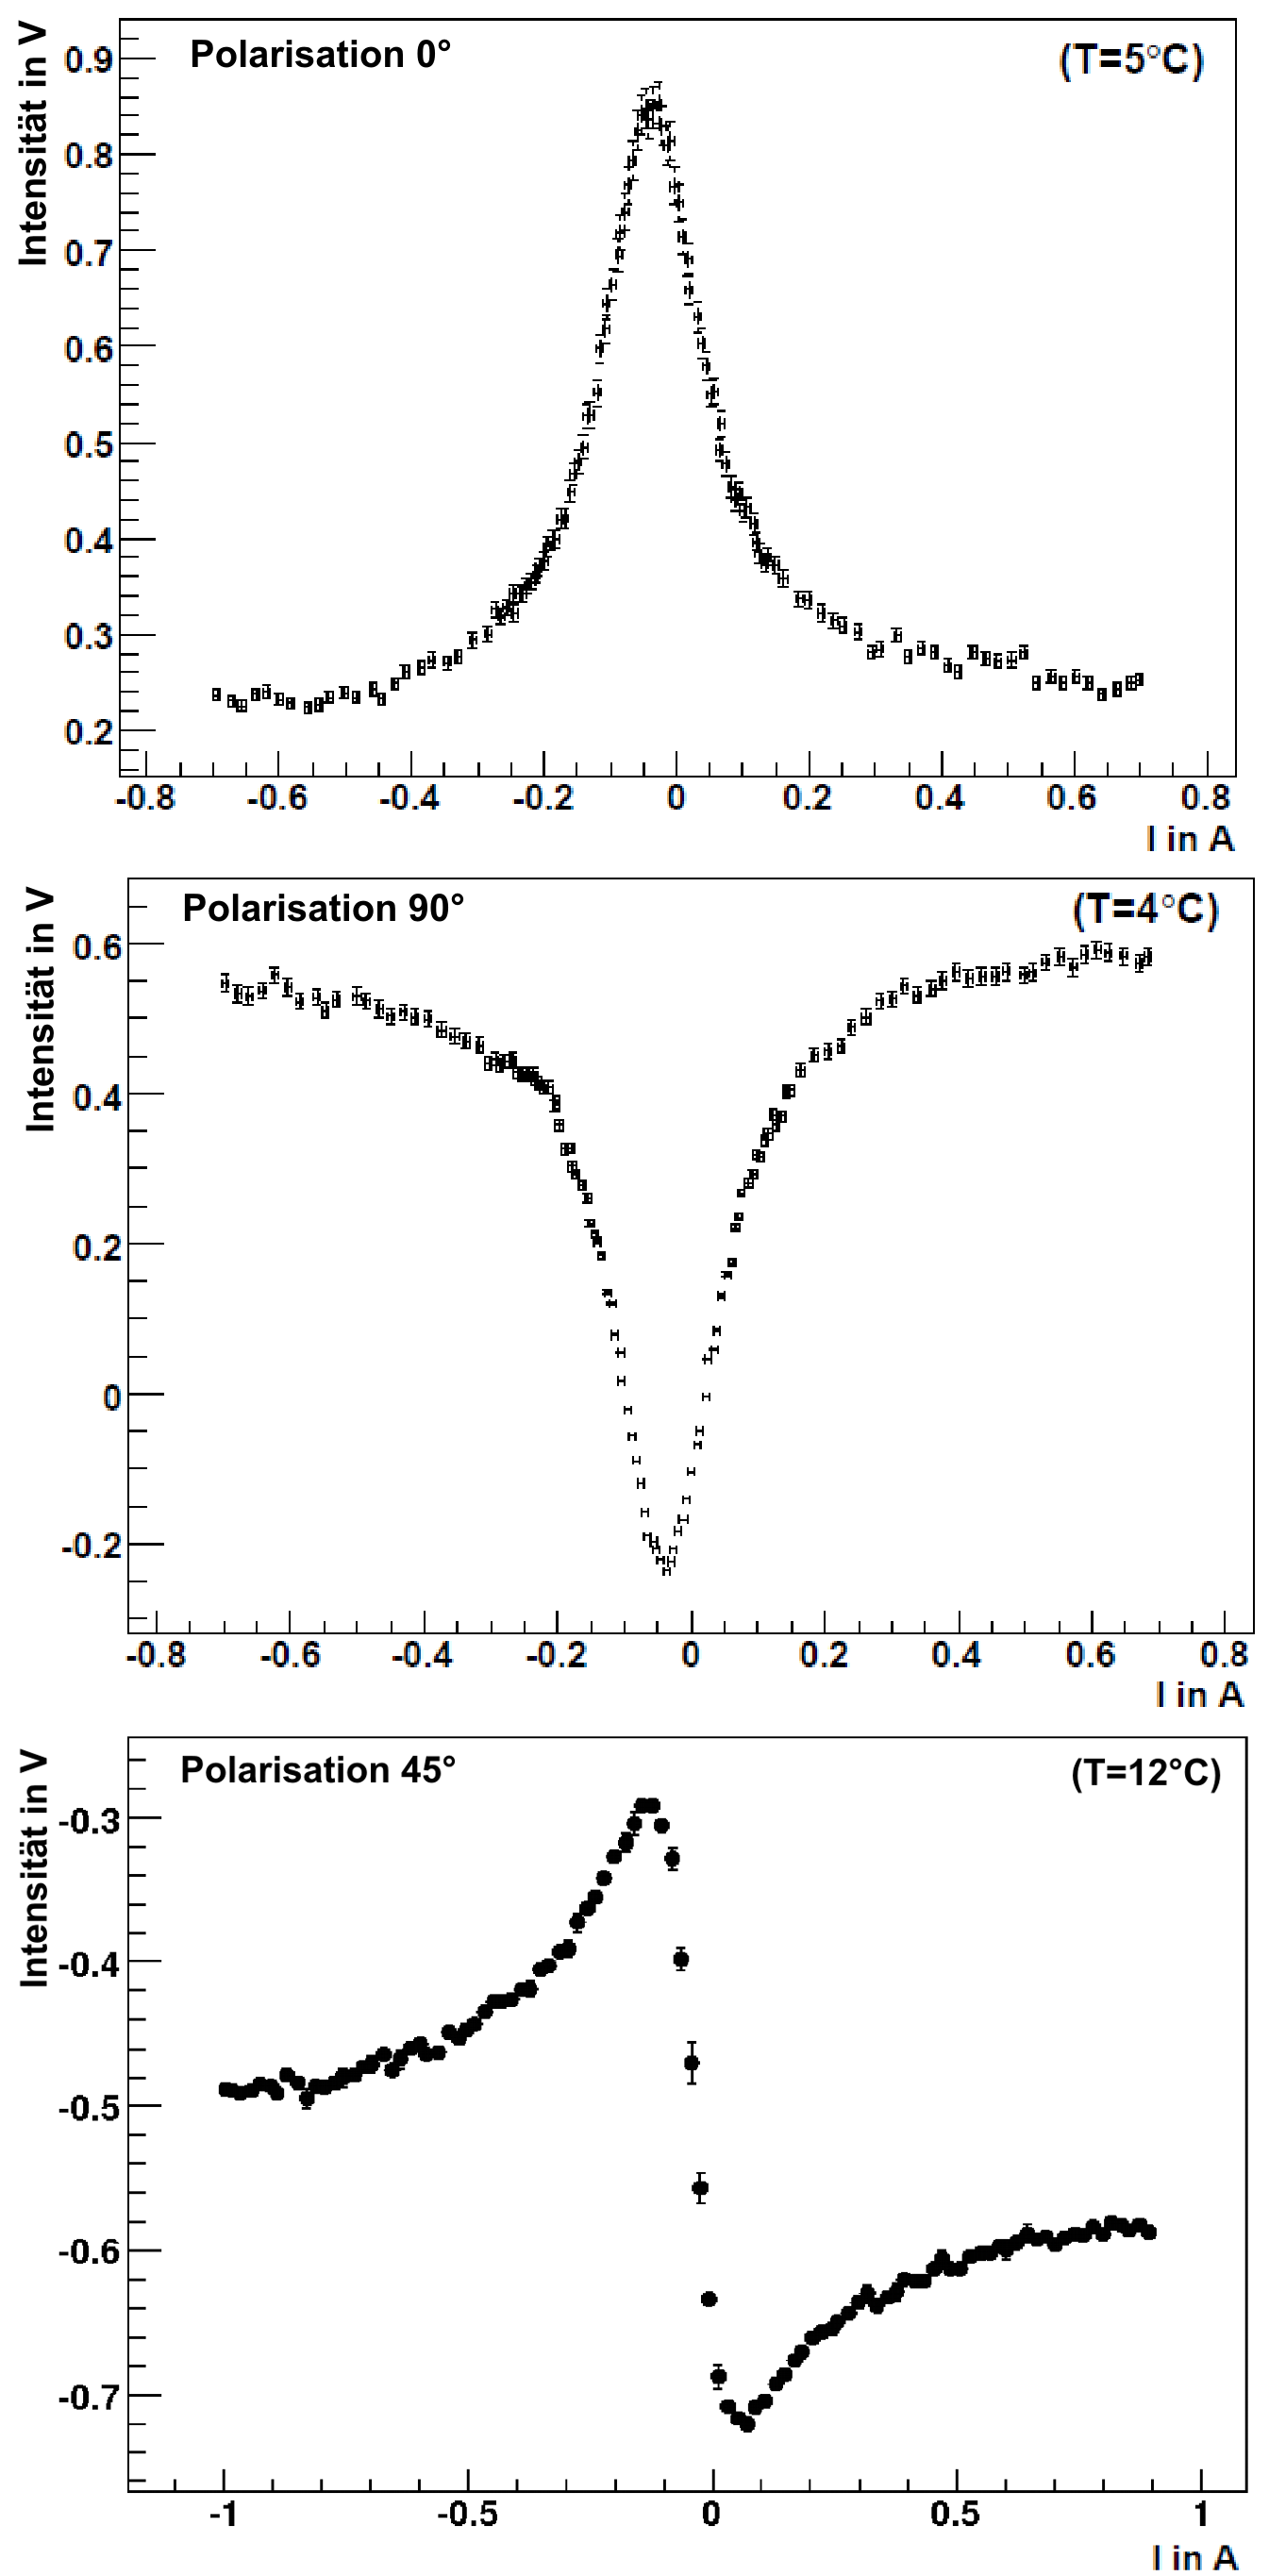
\includegraphics[scale=0.26]{Bilder/signale}
\end{figure}
\end{center}
\clearpage
\subsection{Coherence Narrowing und Dampfdruck}
\subsubsection{Coherence Narrowing}
Durch diesen Effekt erscheint die mittlere Lebensdauer eines Zustandes verlängert. Ein Photon, welches durch die Abregung eines Atoms emittiert wurde, kann ein weiteres Atom anregen. Dies führt zu einer weiteren Abregung und somit erneut zu einem emittierten Photon. Dieser Vorgang kann sich mehrfach wiederholen. Alle so ausgesendeten Photonen haben die gleiche Richtung und Polarisation und sind aus diesem Grund ununterscheidbar. Dies bewirkt die scheinbare Verlängerung der Lebensdauer.\\
Um den Einfluss dieses Effekts vernachlässigen zu können, wird die Lebensdauer für verschiedene Drücke des Gases bestimmt und schließlich auf einen Druck von $0 Pa$ extrapoliert.
\subsubsection{Dampfdruck}
Da die Gas-Dichte innerhalb des Systems nicht gemessen werden kann, muss diese über die Temperatur bestimmt werden. Dazu benutzt man folgende in [ver] gegebene Formel: \[ln(p/p_{c})=(T_{c}/T)\cdot(a_{1}T_{r}+a_{2}T_{r}^{1,89}+a_{3}T_{r}^{2}+a_{4}T_{r}^{8}+a_{5}T_{r}^{8,5}+a_{6}T_{r}^{9})~mit~T_{r}=1-T/T_{C}\]
Dabei gilt: $T_{c}=1764K$ ist die kritische Temperatur und $p_{c}=167MPa$ der kritische Druck. Die Werte der Parameter wurden in [ver] ebenfalls gegeben:\\
\begin{table}[htbp]
\begin{center}
\caption{}
\begin{tabular}{|l|l|l|}
\hline
$a_{1}=-4,57618368$ & $a_{2}=-1,40726277$ & $a_{3}=2,36263541$ \\ \hline
$a_{4}=-31,0889985$ & $a_{5}=58,0183959$ & $a_{6}=,27,6304546$ \\ \hline
\end{tabular}
\end{center}
\end{table}

